\chapter{Modelare si proiectare}

\section{Diagrama de cazuri}
\label{sec:ch3sec1}
 \par Exista un sigur tip de utilizator care poate avea interactiune cu aplicatia, pe viitor se poate dezvolta inca un tip de user acesta avand scopul de a administra tabela cu filme. Fiecare utilizator are un nume unic si o parola pentru a se conecta la aplicatie, acolo unde el poate sa: caute filme, sa isi creeze propia lui lista cu filme, sa dea nota la un film sau sa vada detalii despre un film acolo unde sunt prezente si recomandari pentru filmul respectiv.
		\begin{figure}[htbp]
			\centerline{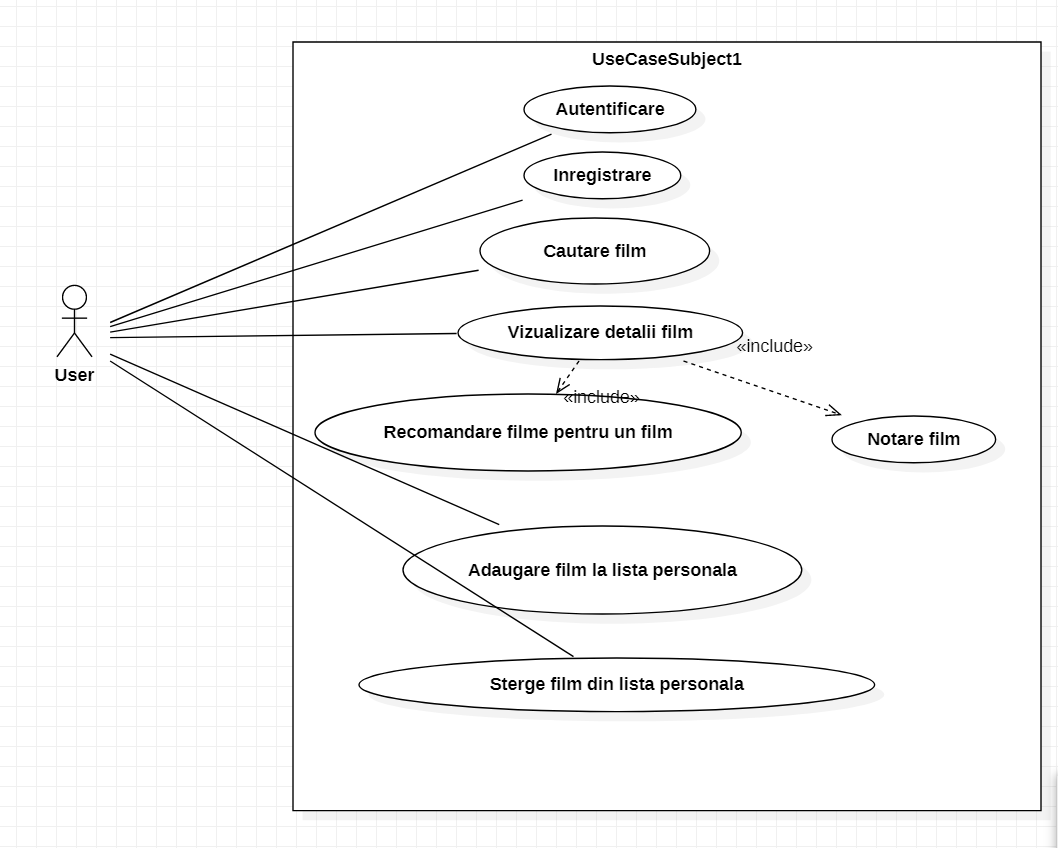
\includegraphics[width=13cm, height=10cm]{figures/use case.png}}
			\caption{Diagrama de cazuri}
			\label{fig}
		\end{figure}



